\documentclass{article}
\usepackage[margin=1in]{geometry}
\usepackage[linesnumbered,ruled,vlined]{algorithm2e}
\usepackage{amsfonts}
\usepackage{amsmath}
\usepackage{amssymb}
\usepackage{amsthm}
\usepackage{enumitem}
\usepackage{fancyhdr}
\usepackage{hyperref}
\usepackage{minted}
\usepackage{multicol}
\usepackage{pdfpages}
\usepackage{standalone}
\usepackage[many]{tcolorbox}
\usepackage{tikz-cd}
\usepackage{transparent}
\usepackage{xcolor}
% \tcbuselibrary{minted}

\author{Nathan Solomon}

\newcommand{\fig}[1]{
    \begin{center}
        \includegraphics[width=\textwidth]{#1}
    \end{center}
}

% Math commands
\renewcommand{\d}{\mathrm{d}}
\DeclareMathOperator{\id}{id}
\DeclareMathOperator{\im}{im}
\DeclareMathOperator{\proj}{proj}
\DeclareMathOperator{\Span}{span}
\DeclareMathOperator{\Tr}{Tr}
\DeclareMathOperator{\tr}{tr}
\DeclareMathOperator{\ad}{ad}
\DeclareMathOperator{\ord}{ord}
%%%%%%%%%%%%%%% \DeclareMathOperator{\sgn}{sgn}
\DeclareMathOperator{\Aut}{Aut}
\DeclareMathOperator{\Inn}{Inn}
\DeclareMathOperator{\Out}{Out}
\DeclareMathOperator{\stab}{stab}

\newcommand{\N}{\ensuremath{\mathbb{N}}}
\newcommand{\Z}{\ensuremath{\mathbb{Z}}}
\newcommand{\Q}{\ensuremath{\mathbb{Q}}}
\newcommand{\R}{\ensuremath{\mathbb{R}}}
\newcommand{\C}{\ensuremath{\mathbb{C}}}
\renewcommand{\H}{\ensuremath{\mathbb{H}}}
\newcommand{\F}{\ensuremath{\mathbb{F}}}

\newcommand{\E}{\ensuremath{\mathbb{E}}}
\renewcommand{\P}{\ensuremath{\mathbb{P}}}

\newcommand{\es}{\ensuremath{\varnothing}}
\newcommand{\inv}{\ensuremath{^{-1}}}
\newcommand{\eps}{\ensuremath{\varepsilon}}
\newcommand{\del}{\ensuremath{\partial}}
\renewcommand{\a}{\ensuremath{\alpha}}

\newcommand{\abs}[1]{\ensuremath{\left\lvert #1 \right\rvert}}
\newcommand{\norm}[1]{\ensuremath{\left\lVert #1\right\rVert}}
\newcommand{\mean}[1]{\ensuremath{\left\langle #1 \right\rangle}}
\newcommand{\floor}[1]{\ensuremath{\left\lfloor #1 \right\rfloor}}
\newcommand{\ceil}[1]{\ensuremath{\left\lceil #1 \right\rceil}}
\newcommand{\bra}[1]{\ensuremath{\left\langle #1 \right\rvert}}
\newcommand{\ket}[1]{\ensuremath{\left\lvert #1 \right\rangle}}
\newcommand{\braket}[2]{\ensuremath{\left.\left\langle #1\right\vert #2 \right\rangle}}

\newcommand{\catname}[1]{{\normalfont\textbf{#1}}}

\newcommand{\up}{\ensuremath{\uparrow}}
\newcommand{\down}{\ensuremath{\downarrow}}

% Custom environments
\newtheorem{thm}{Theorem}[section]

\definecolor{probBackgroundColor}{RGB}{250,240,240}
\definecolor{probAccentColor}{RGB}{140,40,0}
\newenvironment{prob}{
    \stepcounter{thm}
    \begin{tcolorbox}[
        boxrule=1pt,
        sharp corners,
        colback=probBackgroundColor,
        colframe=probAccentColor,
        borderline west={4pt}{0pt}{probAccentColor},
        breakable
    ]
    \color{probAccentColor}\textbf{Problem \thethm.} \color{black}
} {
    \end{tcolorbox}
}

\definecolor{exampleBackgroundColor}{RGB}{212,232,246}
\newenvironment{example}{
    \stepcounter{thm}
    \begin{tcolorbox}[
      boxrule=1pt,
      sharp corners,
      colback=exampleBackgroundColor,
      breakable
    ]
    \textbf{Example \thethm.}
} {
    \end{tcolorbox}
}

\definecolor{propBackgroundColor}{RGB}{255,245,220}
\definecolor{propAccentColor}{RGB}{150,100,0}
\newenvironment{prop}{
    \stepcounter{thm}
    \begin{tcolorbox}[
        boxrule=1pt,
        sharp corners,
        colback=propBackgroundColor,
        colframe=propAccentColor,
        breakable
    ]
    \color{propAccentColor}\textbf{Proposition \thethm. }\color{black}
} {
    \end{tcolorbox}
}

\definecolor{thmBackgroundColor}{RGB}{235,225,245}
\definecolor{thmAccentColor}{RGB}{50,0,100}
\renewenvironment{thm}{
    \stepcounter{thm}
    \begin{tcolorbox}[
        boxrule=1pt,
        sharp corners,
        colback=thmBackgroundColor,
        colframe=thmAccentColor,
        breakable
    ]
    \color{thmAccentColor}\textbf{Theorem \thethm. }\color{black}
} {
    \end{tcolorbox}
}

\definecolor{corBackgroundColor}{RGB}{240,250,250}
\definecolor{corAccentColor}{RGB}{50,100,100}
\newenvironment{cor}{
    \stepcounter{thm}
    \begin{tcolorbox}[
        enhanced,
        boxrule=0pt,
        frame hidden,
        sharp corners,
        colback=corBackgroundColor,
        borderline west={4pt}{0pt}{corAccentColor},
        breakable
    ]
    \color{corAccentColor}\textbf{Corollary \thethm. }\color{black}
} {
    \end{tcolorbox}
}

\definecolor{lemBackgroundColor}{RGB}{255,245,235}
\definecolor{lemAccentColor}{RGB}{250,125,0}
\newenvironment{lem}{
    \stepcounter{thm}
    \begin{tcolorbox}[
        enhanced,
        boxrule=0pt,
        frame hidden,
        sharp corners,
        colback=lemBackgroundColor,
        borderline west={4pt}{0pt}{lemAccentColor},
        breakable
    ]
    \color{lemAccentColor}\textbf{Lemma \thethm. }\color{black}
} {
    \end{tcolorbox}
}

\definecolor{proofBackgroundColor}{RGB}{255,255,255}
\definecolor{proofAccentColor}{RGB}{80,80,80}
\renewenvironment{proof}{
    \begin{tcolorbox}[
        enhanced,
        boxrule=1pt,
        sharp corners,
        colback=proofBackgroundColor,
        colframe=proofAccentColor,
        borderline west={4pt}{0pt}{proofAccentColor},
        breakable
    ]
    \color{proofAccentColor}\emph{\textbf{Proof. }}\color{black}
} {
    \qed \end{tcolorbox}
}

\definecolor{noteBackgroundColor}{RGB}{240,250,240}
\definecolor{noteAccentColor}{RGB}{30,130,30}
\newenvironment{note}{
    \begin{tcolorbox}[
        enhanced,
        boxrule=0pt,
        frame hidden,
        sharp corners,
        colback=noteBackgroundColor,
        borderline west={4pt}{0pt}{noteAccentColor},
        breakable
    ]
    \color{noteAccentColor}\textbf{Note. }\color{black}
} {
    \end{tcolorbox}
}


\fancyhf{}
\setlength{\headheight}{24pt}

\date{\today}
\title{Math 115B Homework \#2}

\begin{document}
\maketitle

\begin{prob}
\end{prob}
\begin{enumerate}[label=(\alph*)]
    \item Let
        \[ u = \begin{bmatrix}
            u_1 \\
            u_2 \\
            u_3
        \end{bmatrix} \]
        be an arbitrary vector in $V$. Then the dual basis $\mathcal{B}^*$ consists of the following linear functionals:
        \begin{align*}
            u &\mapsto u_1 - 2^{-1} u_2 \\
            u &\mapsto 2^{-1} u_2 \\
            u &\mapsto u_3 - u_1.
        \end{align*}
        This was obtained by finding the following inverse matrix:
        \[ \begin{bmatrix}
            1 & 1 & 0 \\
            0 & 2 & 0 \\
            1 & 1 & 1
        \end{bmatrix}^{-1} = \begin{bmatrix}
            1 & - \frac{1}{2} & 0 \\
            0 & \frac{1}{2} & 0 \\
            -1 & 0 & 1
        \end{bmatrix}. \]
    \item Given an arbitrary element $u = u_2 x^2 + u_1 x + u_0 \in V$, the dual basis $\mathcal{B}^*$ consists of the following 3 linear functionals: \begin{align*}
            u &\mapsto u_0 = u(0) \\
            u &\mapsto u_1 = u'(0) \\
            u &\mapsto u_2 = 2^{-1} u''(0).
    \end{align*}
\end{enumerate}

\bigskip
\par
\begin{prob}
\end{prob}
\begin{enumerate}[label=(\alph*)]
    \item $T*f$ is the functional which maps $ \begin{bmatrix}
        x \\
        y
    \end{bmatrix}$ to
    \[ T*f \begin{bmatrix}
        x \\
        y
    \end{bmatrix} = fT \begin{bmatrix}
        x \\
        y
    \end{bmatrix} = f \begin{bmatrix}
        3x+2y \\
        x
    \end{bmatrix} = 2(3x+2y)+(x) = 7x+4y. \]
    \item For this problem, I will represent all transformations in the standard basis $\varepsilon$ and its dual, $\varepsilon^*$.
        \par
        You can think of $f$ as the row vector $ \begin{bmatrix}
            2 & 1
    \end{bmatrix}$, and $T$ as the matrix
    \[ T := \begin{bmatrix}
        3 & 2 \\
        1 & 0
    \end{bmatrix}. \]
    $T^*$ can be represented by the transpose of $T$,
    \[ T^* = \begin{bmatrix}
        3 & 1 \\
        2 & 0
    \end{bmatrix} \]
    By looking at the matrix representation I already found for $T^*$ in the dual of the standard basis, we can see $a=3, b=1, c=2, d=0$.
\item \begin{align*}
        [T]_\varepsilon &= \begin{bmatrix}
            3 & 2 \\
            1 & 0
        \end{bmatrix} \\
            ([T]_\varepsilon)^T &= \begin{bmatrix}
            3 & 1 \\
            2 & 0
        \end{bmatrix} = [T^*]_{\varepsilon^*}.
\end{align*}
\end{enumerate}

\bigskip
\par
\begin{prob}
\end{prob}
\begin{enumerate}[label=(\alph*)]
    \item Let $f,g$ be arbitrary elements of $S^0$, and let $c$ be an arbitrary element of $k$. Then $f+cg \in V^*$, and for all $x \in S$,
        \[ (f+cg)(x) = f(x)+cg(x) = 0+0c=0, \]
        so $f+cg \in S^0$, and $S^0$ also contains the zero funcitonal, which means $S^0$ is a subspace of $V^*$.
    \item Since $V$ is finite dimensional and $x \neq 0$, there exists some basis $\mathcal{B}$ of $V$ which contains $x$ and contains a subset which spans $W$. Any vector $v \in V$ can be written as a finite sum of scalars in $k$ times basis vectors in $\mathcal{B}$, so there exists a linear functional $f$ which maps $v$ to the coefficient of $x$ in that sum. Since $f$ maps all basis vectors of $W$ to zero, $f$ is in $W^0$. Lastly, note that $f(x)=1\neq 0$.
    \item Let $(x_1, \dots, x_n, y_1, \dots, y_m)$ be a basis for $V$ such that $(x_1, \dots, x_n)$ is a basis for $S$. Then $(y_1^*, \dots, y_m^*)$ is a basis for $S^0$. By that same reasoning, $(x_1^{**}, \dots, x_n^{**})$ is a basis for $(S^0)^0$. The span of that last basis is equal to $\Span(\psi(S))$.
    \item If $W_1 \neq W_2$, then without loss of generality, there exists $x \in W_1$ such that $x \not\in W_2$. That implies there exists $f \in W_2^0$ such that $f(x) \neq 0$, but $f \not\in W_1^0$, so $W_1^0 \neq W_2^0$.
        \par
        If $W_1^0 \neq W_2^0$, then $(W_1^0)^0 \neq (W_2^0)^0$, which means $\Span(\psi(W_1)) \neq \Span(\psi(W_2))$. Both $\psi(W_1)$ and $\psi(W_2)$ are subspaces, so $\psi(W_1)\neq \psi(W_2)$. $\psi$ is an isomorphism, so $W_1 \neq W_2$.
        \par
        I have shown that $W_1 \neq W_2$ implies $W_1^0 \neq W_2^0$ and vice versa, so $W_1 = W_2$ iff $W_1^0 = W_2^0$.
    \item A functional $f \in V^*$ is in $(W_1 + W_2)^0$ iff $f(w_1+w_2)=f(w_1)+f(w_2)=0$ for any $w_1 \in W_1, w_2 \in W_2$. That is true iff $f(w_1)=0$ for any $w_1 \in W_1$ and $f(w_2)=0$ for any $w_2 \in W_2$. This is equivalent to saying $f \in W_1^0$ and $f \in W_2^0$, which is equivalent to saying $f \in W_1^0 \cap W_2^0$.
\end{enumerate}

\bigskip
\par
\begin{prob}
\end{prob}
Dimension is defined as the cardinality of a basis, so in order for that to be defined, I will assume for now that every vector space has a basis.
\par
Let $\mathcal{B}_W$ be a basis of $W$, and extend that to a basis $\mathcal{B}_V$ for $V$ -- in other words, when choosing a basis, make sure that $\mathcal{B}_W \subset \mathcal{B}_V$. Then each element of $\mathcal{B}_W^*$ will map the corresponding basis vector in $\mathcal{B}_W$ to a nonzero value, so none of the dual vectors in $\mathcal{B}_W^*$ are in $W^0$. However, every dual basis vector in $\mathcal{B}_V^* \backslash \mathcal{B}_W^*$ will map all elements of $\mathcal{B}_W$ to zero. If $\dim(W^0)$ is finite, then $\mathcal{B}_V^* \backslash \mathcal{B}_W^*$ is a basis for $W^0$. We now have
\begin{align*}
    \dim(W) + \dim(W^0) &= \abs{\mathcal{B}_W} + \abs{\mathcal{B}_V^* \backslash \mathcal{B}_W^*} \\
                        &= \abs{\mathcal{B}_V} \\
                        &= \dim(V).
\end{align*}
If $\dim(W^0)$ is infinite, I'm not sure how to solve this problem.

\bigskip
\par
\begin{prob}
\end{prob}
If $g \in \ker(T^*)$, then for any $v \in V$, we have $T^*gv = 0$, but we also know $T^*(g) = g \circ T$, so $0 = (g \circ T)(v) = g(Tv)$. Every element of $R(T)$ can be written as $Tv$ for some $v \in V$, so $g$ maps every element of $R(T)$ to zero, which means $\ker(T^*) \subset R(T)^0$.
\par
This also works in reverse -- if $g \in R(T)^0$, then for any $v \in W$, we can let $u=Tv$, and since $u \in R(T)$, $g(u)=0$. Equivalently, $(g \circ T)(v) = 0$, which means $(T^*(g))(v)=0$, so $g \in \ker(T^*)$. That means $R(T)^0 \subset \ker(T^*)$, so $R(T)^0 = \ker(T^*)$.

\bigskip
\par
\begin{prob}
\end{prob}
The characteristic polynomial is
\begin{align*}
    \det (R - \lambda I) &= \det \left( \begin{bmatrix}
            -3-\lambda & -3 & -4 \\
            2 & 2 - \lambda & 4 \\
            0 & 0 & -1 - \lambda
    \end{bmatrix} \right) \\
                         &= (-3-\lambda)(2-\lambda)(-1-\lambda) - (-3)(2)(-1-\lambda) \\
                         &= (6+5\lambda-2\lambda^2-\lambda^3)-(6+6\lambda) \\
                         &= -\lambda^3-2\lambda^2-\lambda \\
                         &= -\lambda(\lambda+1)^2.
\end{align*}
The roots of that are $\lambda = 0$ (with multiplicity 1, so the corresponding eigenspace is 1D) and $\lambda = -1$ (with multiplicity 2, so the corresponding eigenspace is 2D).
\par
The $\lambda=0$ eigenspace is the nullspace of $R$, which is
\[ \Span \left( \begin{bmatrix}
    1 \\
    -1 \\
    0
\end{bmatrix} \right) \]
and the $\lambda=-1$ eigenspace is the nullspace of
\[ R-(-1)I=R+I = \begin{bmatrix}
    -2 & -3 & -4 \\
    2 & 3 & 4 \\
    0 & 0 & 0
\end{bmatrix}, \]
which is
\[ \Span \left( \begin{bmatrix}
    3 \\
    -2 \\
    0
\end{bmatrix}, \begin{bmatrix}
    2 \\
    0 \\
    -1
\end{bmatrix} \right). \]


\bigskip
\par
\begin{prob}
\end{prob}
In the standard basis $\varepsilon$,
\[ [T]_\varepsilon = \begin{bmatrix}
    4 & -1 \\
    2 & 1
\end{bmatrix}, \]
which has eigenvectors $ v_1 := \begin{bmatrix}
    1 \\
    1
\end{bmatrix}$ (with eigenvalue 3) and $ v_2 := \begin{bmatrix}
    1 \\
    2
\end{bmatrix}$ (with eigenvector 3). This means in the basis $\mathcal{B} := (v_1, v_2)$, $T$ is diagonal:
\[ [T]_\mathcal{B} = \begin{bmatrix}
    3 & 0 \\
    0 & 2
\end{bmatrix}. \]
This works because $Tv_1=3v_1$ and $Tv_2=2v_2$.

\bigskip
\par
\begin{prob}
\end{prob}
\begin{enumerate}[label=(\alph*)]
    \item This is $T$-invariant, because the derivative of any polynomial with degree less than or equal to 2 will be another polynomial with degree less than or equal to 2.
    \item This is not $T$-invariant, because $x^2 \in W$, but $T(x^2)=x^3 \not\in W$.
    \item This is $T$-invariant, because for any vector in the image of $T$, all 3 components of that vector are the same, which means the vector is in $W$.
    \item This is $T$-invariant, because if $f\in W$ is the function which maps any $t \in [0,1]$ to $at+b$, then $Tf$ is the function which maps $t \in [0,1]$ to
        \[ \left( \int_0^1 f(x) \d x \right) t = \left[ \frac{a}{2} x^2 + bx \right]_{x=0}^1 t = (b+a/2)t, \]
        which is a linear function of $t$. Since $T$ maps any affine function $f(t)=at+b$ to another affine function $(Tf)(t)=(b+a/2)t$, $W$ is a $T$-invariant subspace.
    \item This is not $T$-invariant, because any symmetric $2 \times 2$ matrix $A$ can be written as
        \[ A = \begin{bmatrix}
            a & b \\
            b & c
        \end{bmatrix}. \]
        which means
        \[ TA = \begin{bmatrix}
            b & c \\
            a & b
        \end{bmatrix}, \]
        which is not symmetric when $a=0$ and $c=1$.
\end{enumerate}


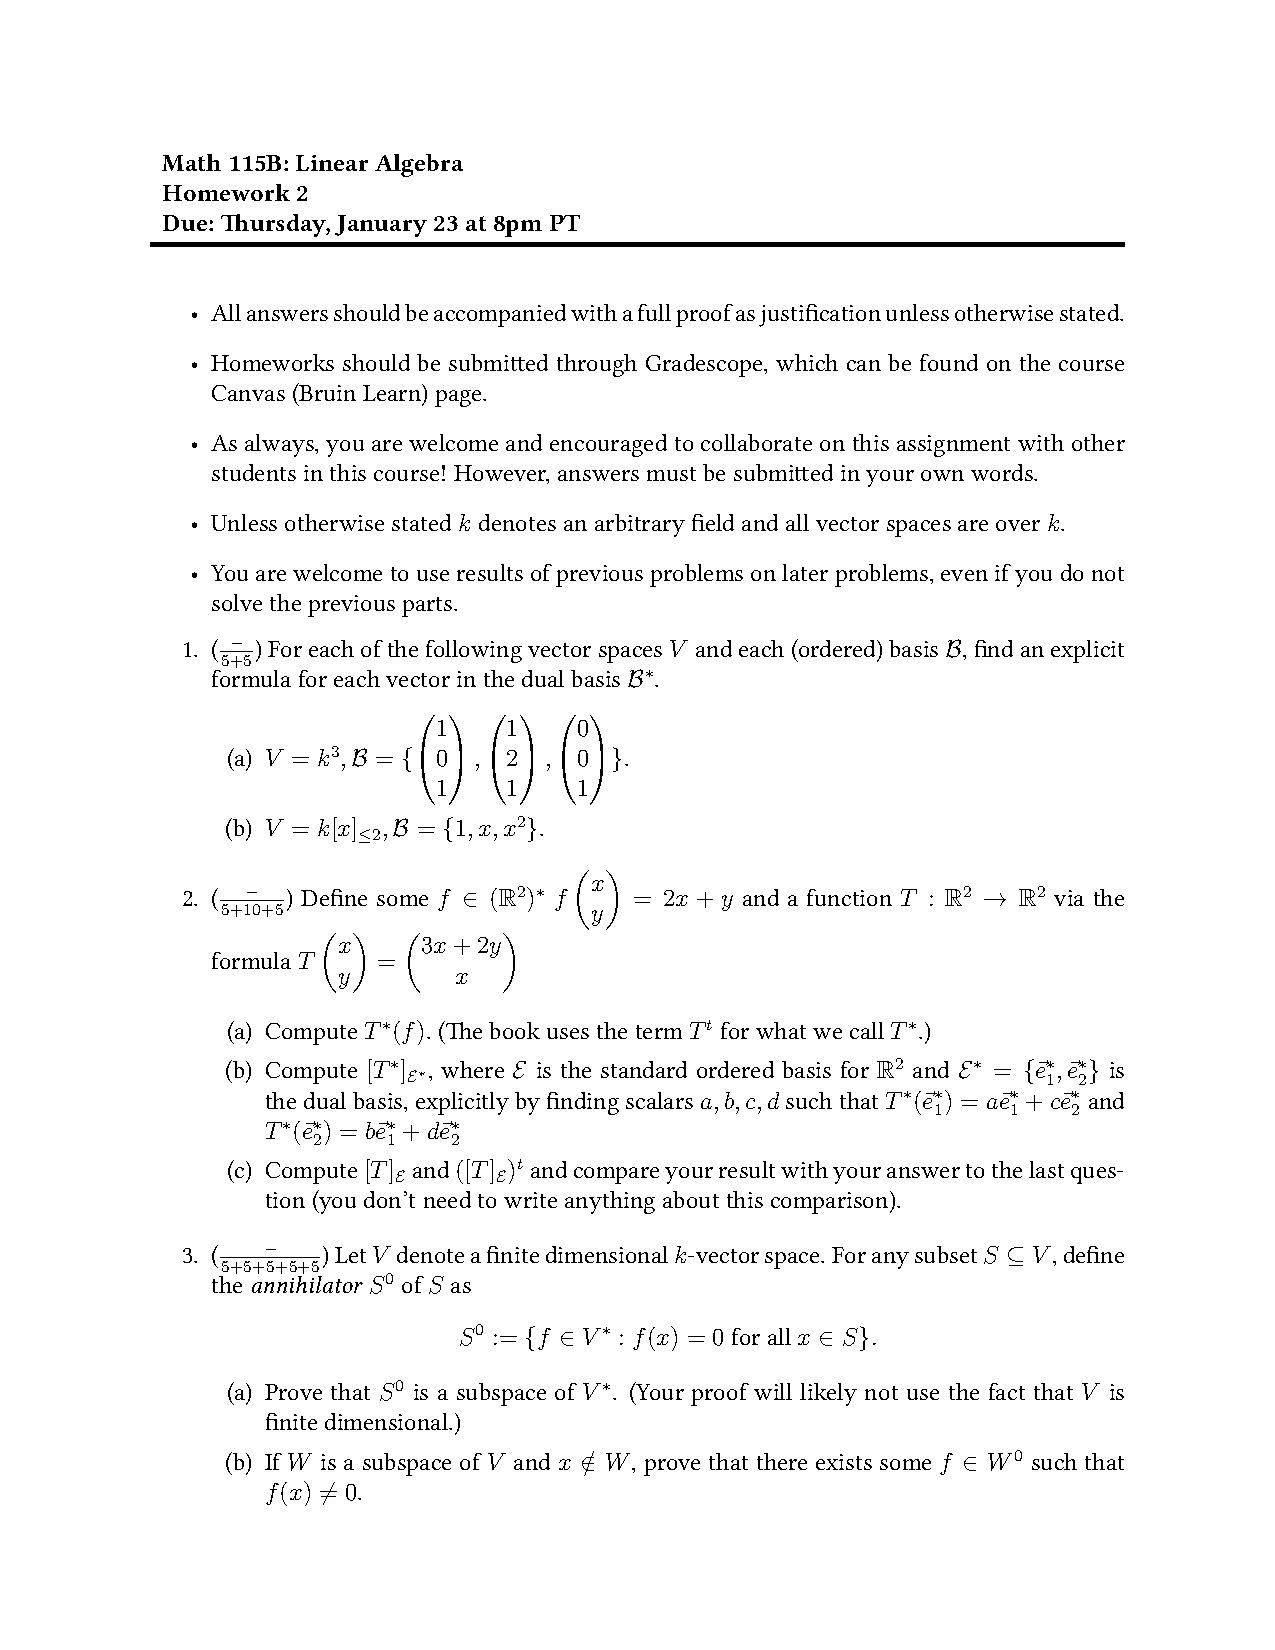
\includepdf[pages=-]{assignment.pdf}

\end{document}
